\begin{figure}[p]
\centering
\makebox[\textwidth][c]{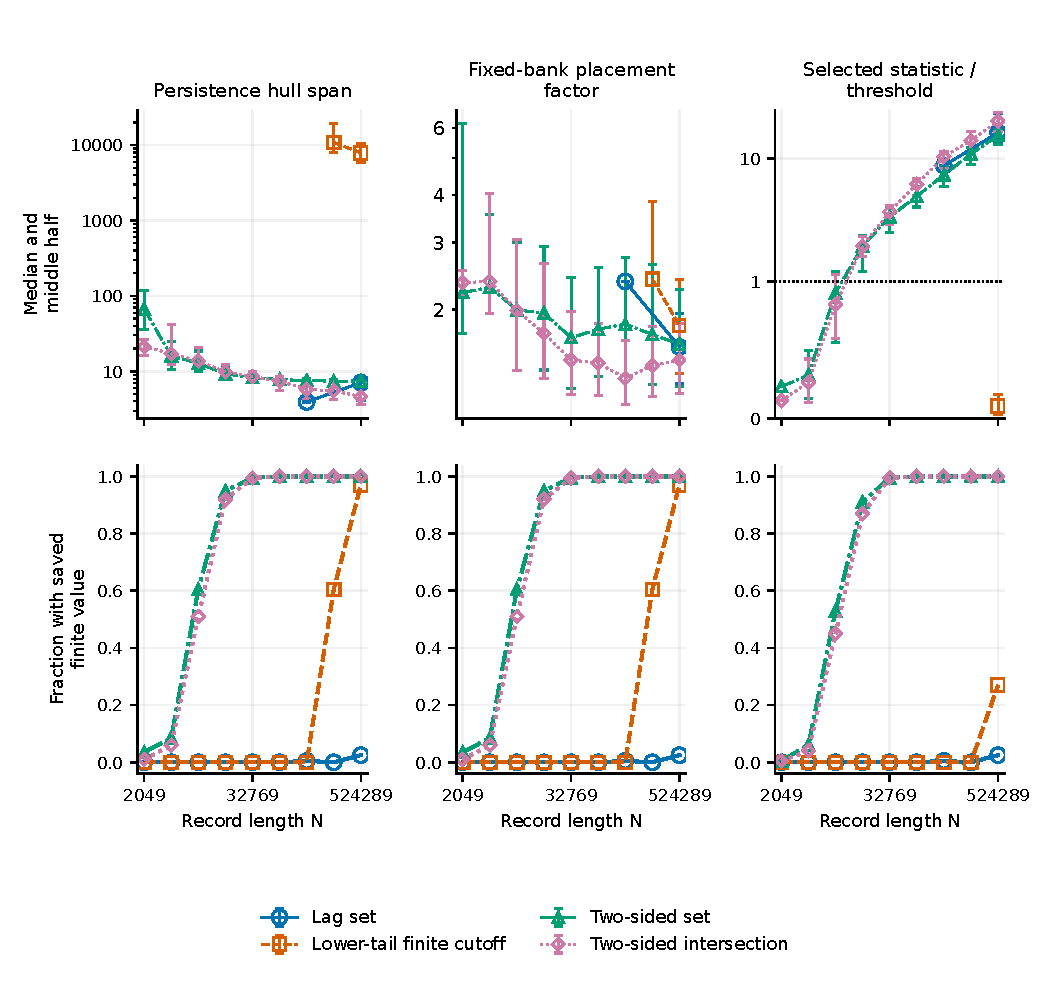
\includegraphics[width=7in]{figures/source_hull_bank_threshold.pdf}}
\caption{Finite source geometry and an available threshold occur on different record subsets. At $\phi=0.995$, each length has 200 records. Upper panels show finite-value medians and interquartile ranges; lower panels show finite-value fractions. The first two upper axes are logarithmic; the third is linear through one and logarithmic above it. Missing values are omitted, not zero. Section~\ref{sec:src16:diagnostic-definitions} defines the summaries.}\label{fig:src16:hull-bank-threshold}
\end{figure}

\begin{figure}[p]
\centering
\makebox[\textwidth][c]{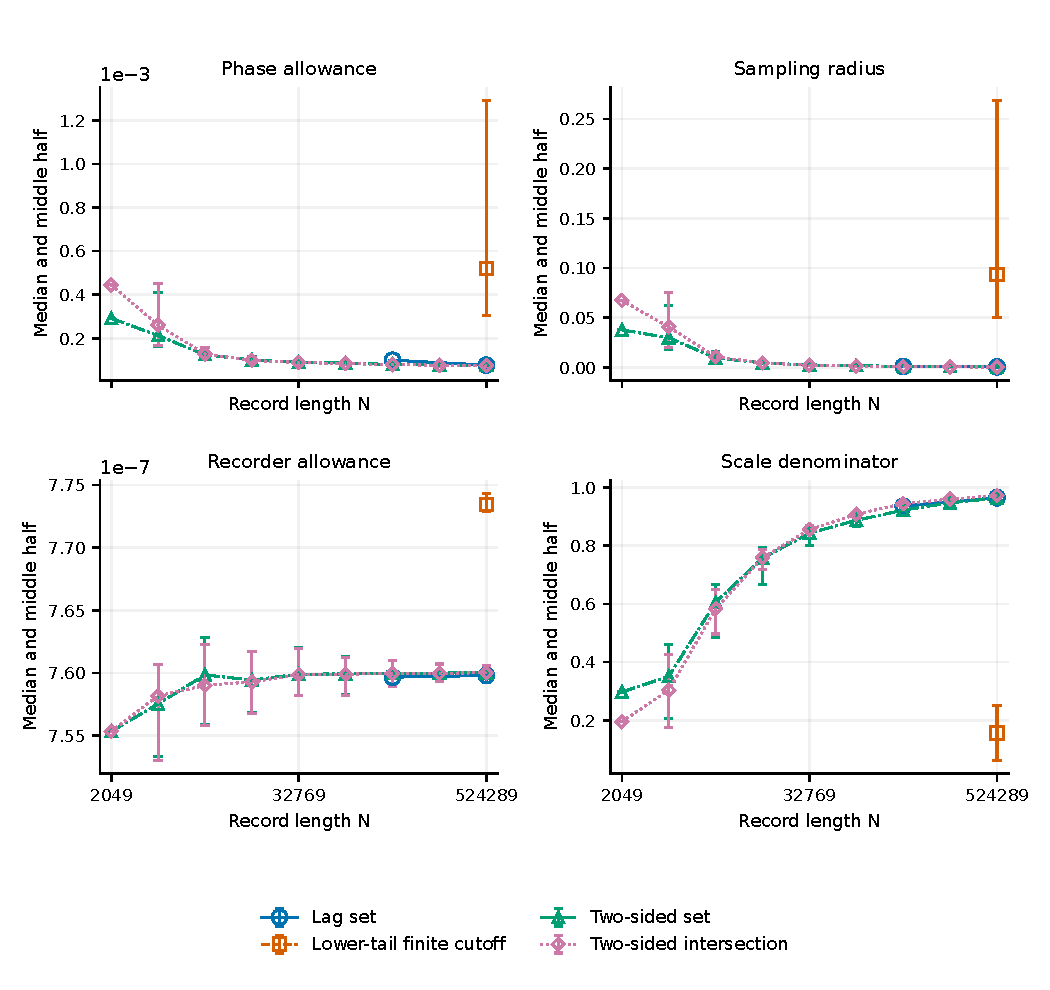
\includegraphics[width=6.8in]{figures/source_threshold_components.pdf}}
\caption{Median sampling allowances remain larger than median phase allowances in the selected two-sided members. At $\phi=0.995$, each length has 200 records. Curves give medians and interquartile ranges of saved finite values for the member with largest statistic-minus-threshold margin. Allowances use upper endpoints and denominators use lower endpoints. These ranges are descriptive, not confidence intervals. Missing values are omitted; a median total need not equal summed medians.}\label{fig:src16:threshold-components}
\end{figure}

\begin{figure}[p]
\centering
\makebox[\textwidth][c]{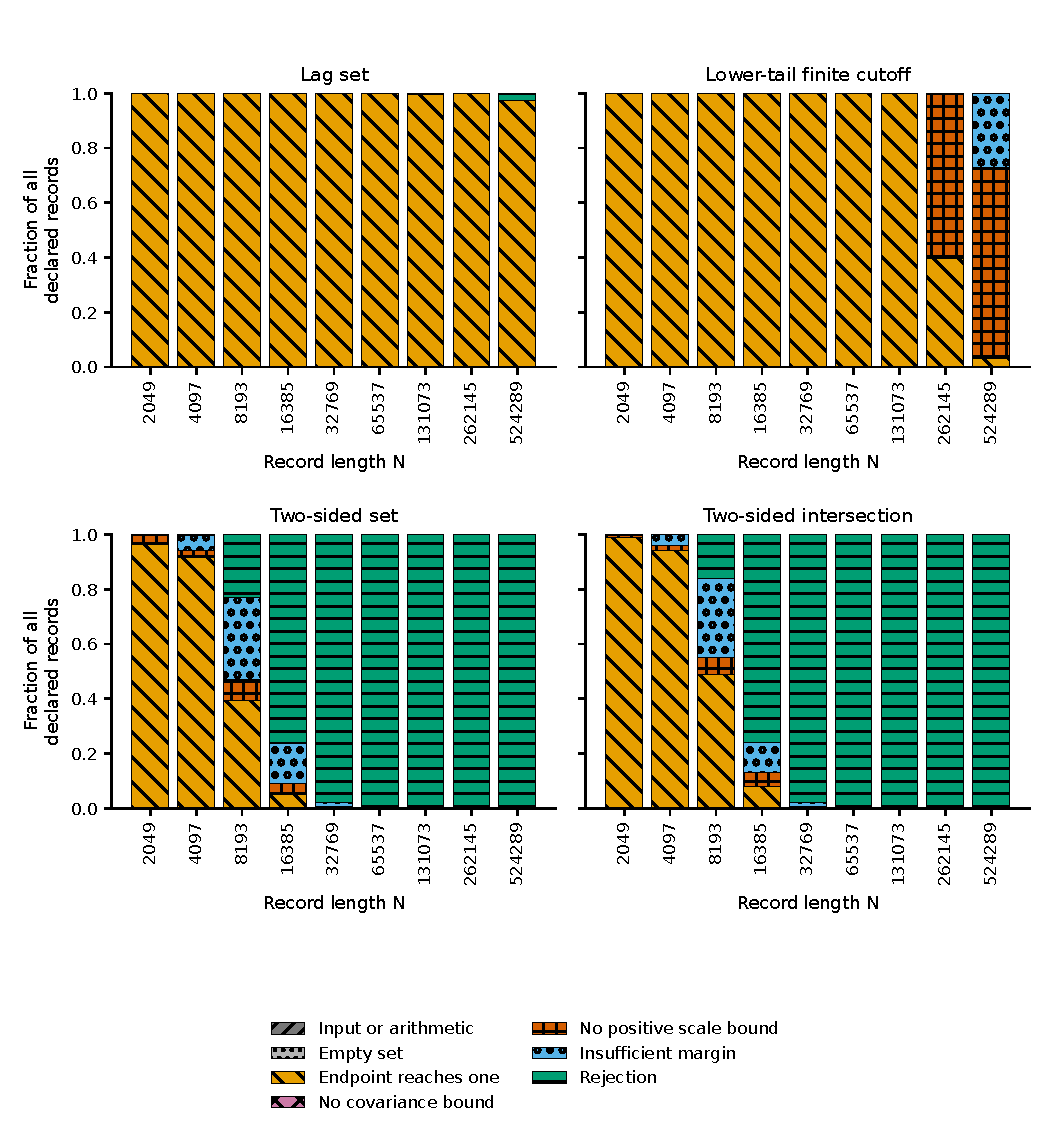
\includegraphics[width=7in]{figures/source_first_failure.pdf}}
\caption{The first failed condition separates unavailable tests from available nonrejections. Each bar uses all 200 records at one strong-delay length, with $\phi=0.995$. Seven mutually exclusive categories cover failures, nonrejections, and rejections, as defined in Sec.~\ref{sec:src16:first-failure}. A first failure does not imply that later requirements passed. Fractions are descriptive and carry no confidence intervals.}\label{fig:src16:first-failure}
\end{figure}

\begin{figure}[p]
\centering
\makebox[\textwidth][c]{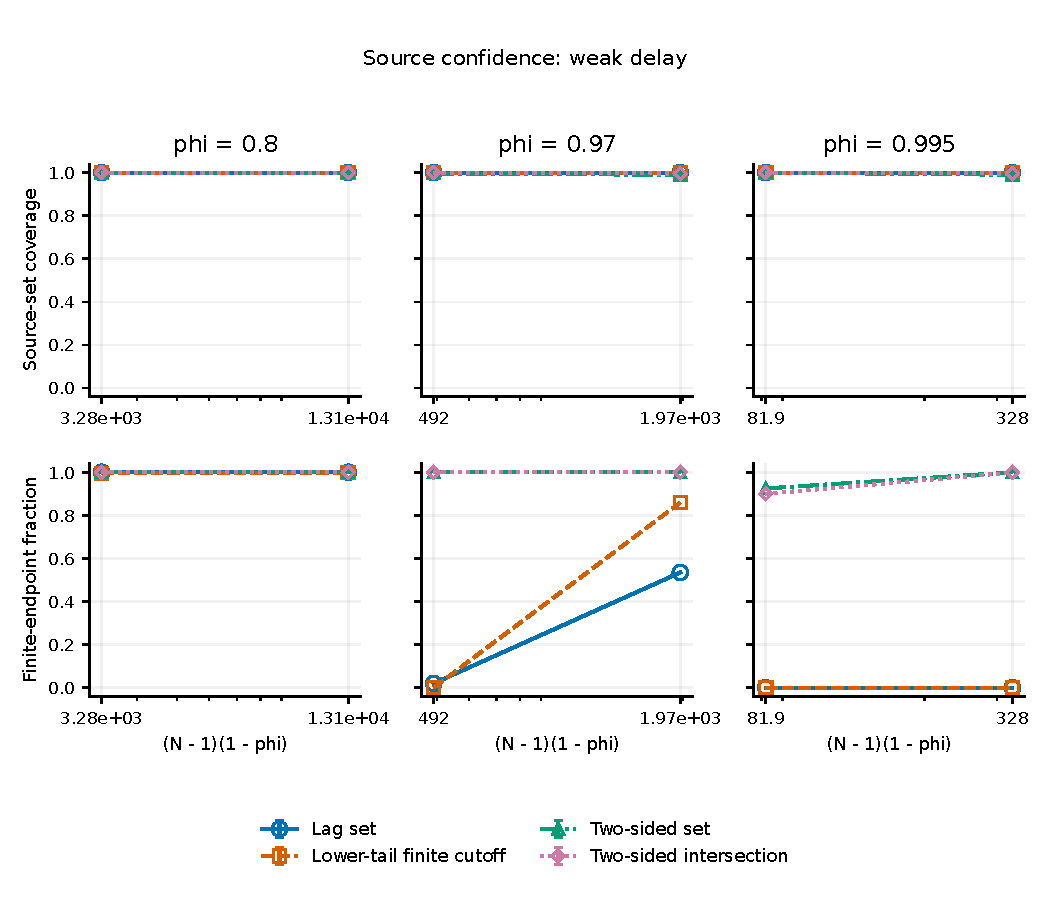
\includegraphics[width=7in]{figures/source_confidence_weak.pdf}}
\caption{Weak-delay source coverage and endpoint availability can differ sharply. Each cell has 200 records. Coverage bars are pointwise 95\% binomial intervals. Coverage and finite-endpoint fractions use the complete sample, while the confidence-set error allowance is $0.005$. At $\phi=0.995$, lag and lower-tail methods cover every source value but have no finite endpoint at either length. Coincident curves indicate equal fractions.}\label{fig:src16:source-confidence-weak}
\end{figure}
